\chapter{Sprints} \label{appendix:sprints}

\subimport{}{sprint-0.tex}

\section*{Total und Fazit}

\xxx[Daten eintragen]

\begin{table}[H]
	\centering
	\begin{tabular}{ll}
		\toprule
		\multicolumn{2}{l}{\textbf{Total}}\\
		\midrule
		\textbf{Periode} & 22.02.2016\textendash xx.06.2016\\
		\textbf{Stunden Soll} & \SI{000}{\hour}\\
		\textbf{Stunden Ist} & \SI{000}{\hour}\\
		\bottomrule
	\end{tabular}
\end{table}

\begin{table}[H]
	\centering
	\begin{tabular}{ll}
		\toprule
		\multicolumn{2}{l}{\textbf{Total pro Person}}\\
		\midrule
		\textbf{Ueli Bosshard} & \SI{000}{\hour}\\
		\textbf{Philipp Christen} & \SI{000}{\hour}\\
		\bottomrule
	\end{tabular}	
\end{table}

\subsection*{Github commits}

https://github.com/upd89/controlcenter/graphs/contributors

\begin{figure}
  \centering
    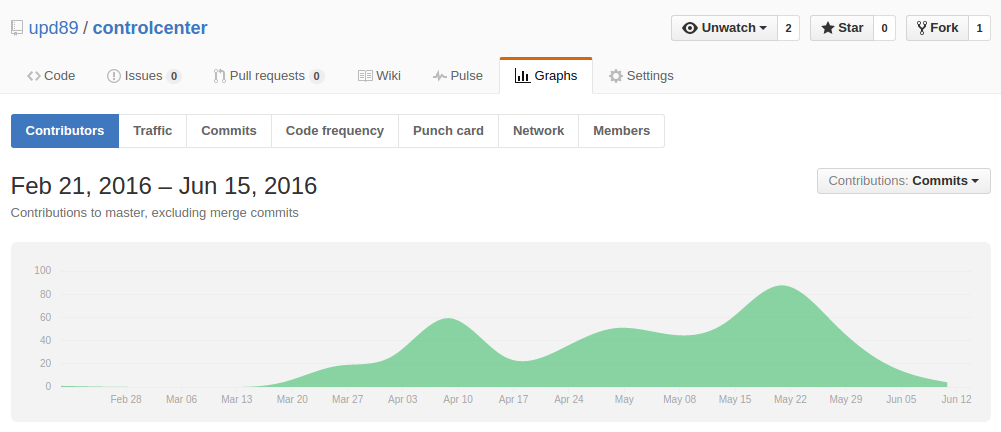
\includegraphics[width=0.95\textwidth]{fig/controlcenter_commits}
  \caption{Anzahl Commits im Control Center}
  \label{fig:commits-cc}
\end{figure}

https://github.com/upd89/agent/graphs/contributors

\begin{figure}
  \centering
    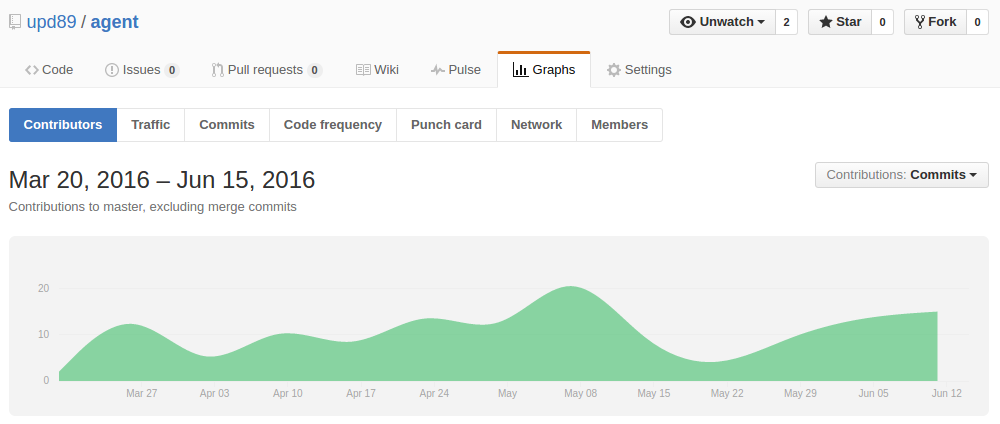
\includegraphics[width=0.95\textwidth]{fig/agent_commits}
  \caption{Anzahl Commits im Agent}
  \label{fig:commits-a}
\end{figure}

\subsection*{Auswertung Redmine}

\begin{figure}
  \centering
    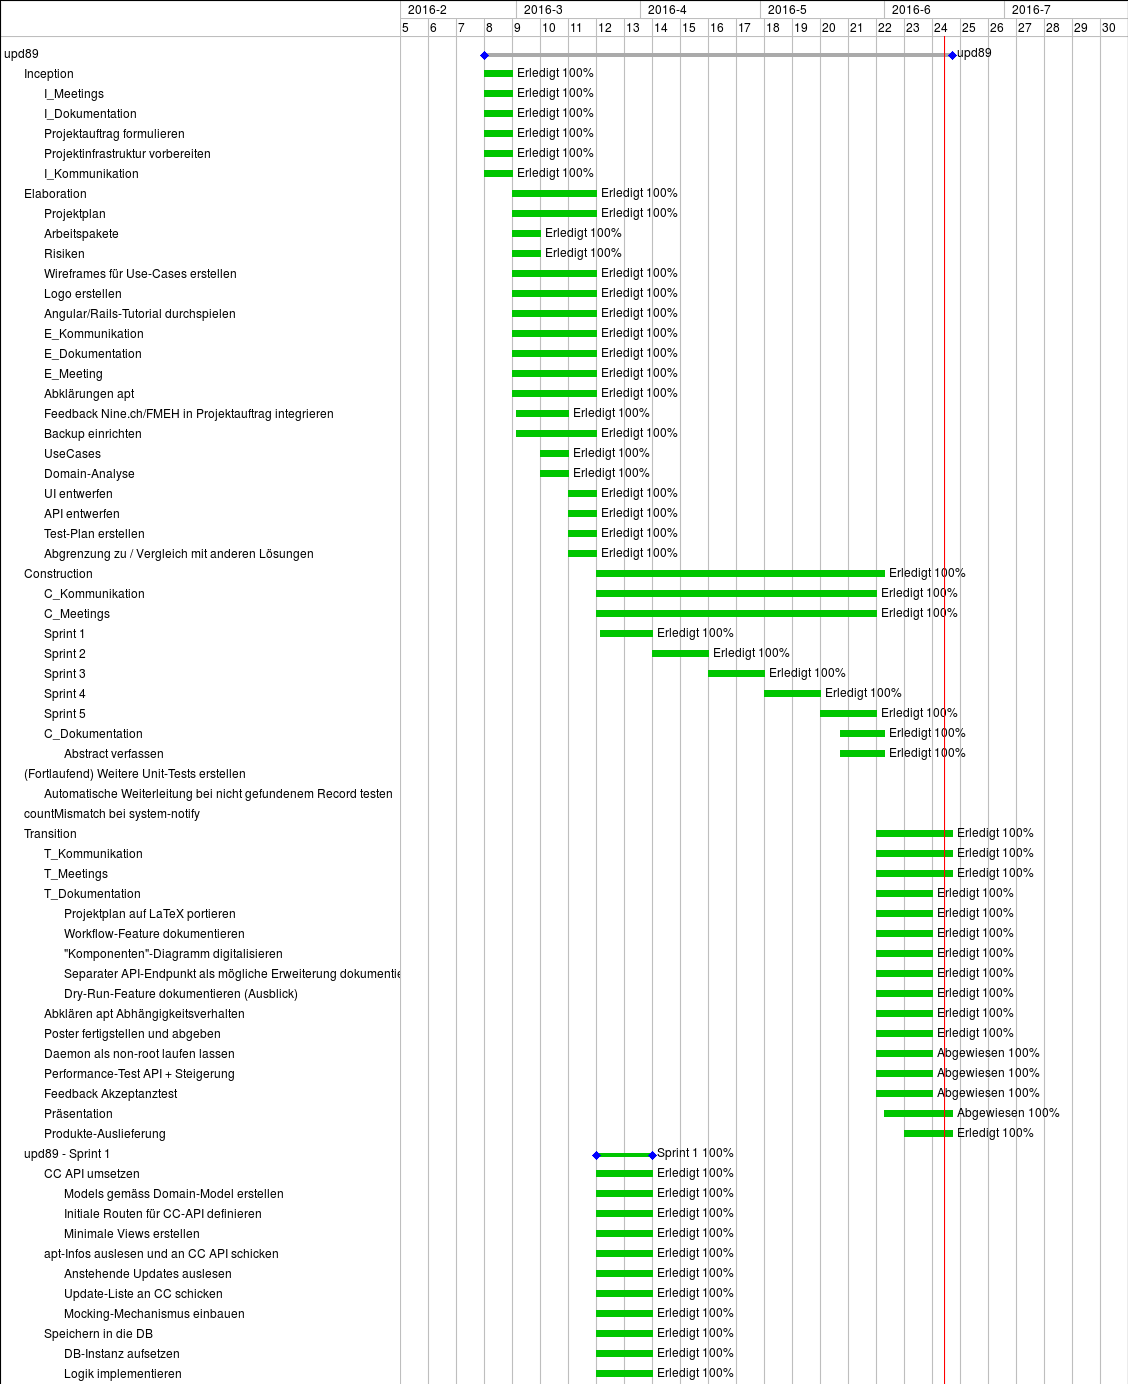
\includegraphics[width=0.95\textwidth]{fig/upd89-gantt-part1}
  \caption{Finales Grantt-Diagram 1/2}
  \label{fig:gantt-final1}
\end{figure}

\begin{figure}
  \centering
    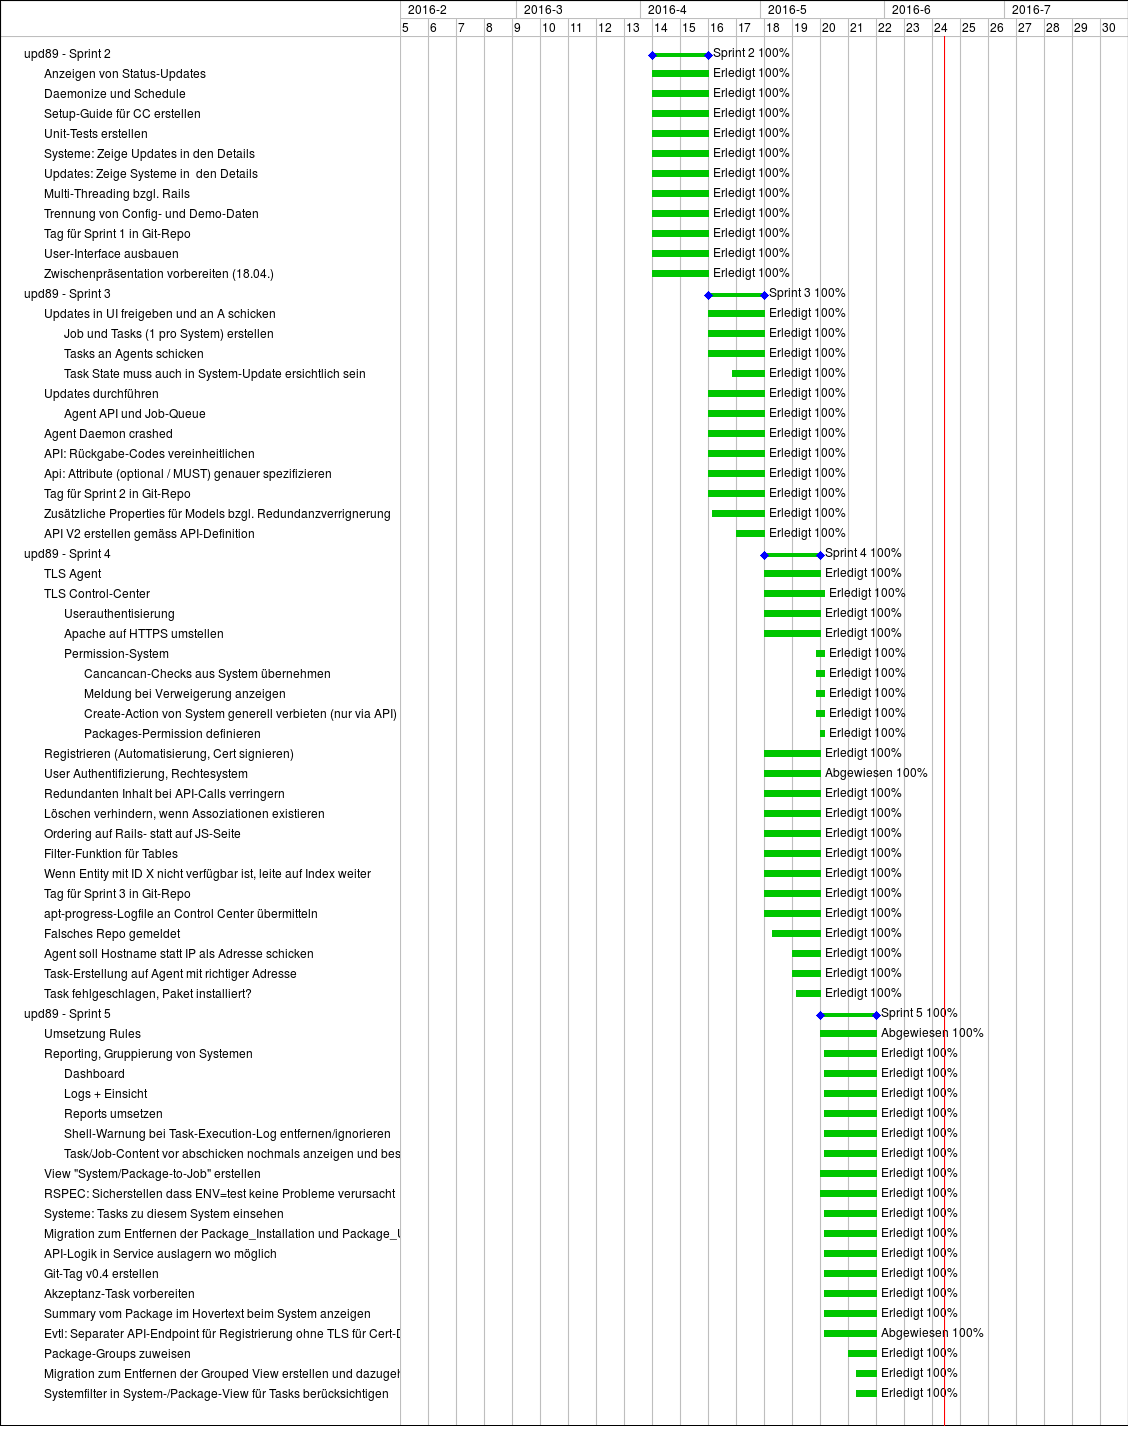
\includegraphics[width=0.95\textwidth]{fig/upd89-gantt-part2}
  \caption{Finales  Grantt-Diagram 2/2}
  \label{fig:gantt-final2}
\end{figure}


\subsubsection*{Stunden pro Woche}

\subsubsection*{Redmine-Tasks}

